
\documentclass[11pt,oneside]{article} 

\usepackage{a4wide}

\usepackage{amsmath}
\usepackage{color}
%\usepackage{natbib} % kills arxiv 
\usepackage{framed}
%\usepackage{cite}
\usepackage{tikz}
\usepackage{tikz-cd}

\RequirePackage{amsmath}
\RequirePackage{amssymb}
\RequirePackage{amsthm}
%\RequirePackage{algorithmic}
%\RequirePackage{algorithm}
%\RequirePackage{theorem}
%\RequirePackage{eucal}
\RequirePackage{color}
\RequirePackage{url}
\RequirePackage{mdwlist}

\RequirePackage{rotating}


\RequirePackage[all]{xy}
%\_CompileMatrices
%\RequirePackage{hyperref}
\RequirePackage{graphicx}
%\RequirePackage[dvips]{geometry}

\usepackage{xcolor}
\usepackage{amsmath,amsfonts,amssymb}
\usepackage{graphicx}
\usepackage[caption=false]{subfig}
\usepackage{enumerate}
\usepackage{mathrsfs}
\usepackage{mathtools}

% -------------- _Commands ----------------------

\makeatletter
\newcommand{\verbatimfont}[1]{\renewcommand{\verbatim@font}{\ttfamily#1}}
\makeatother

\newcommand{\Eref}[1]{(\ref{#1})}
\newcommand{\Fref}[1]{Fig.~\ref{#1}}
%\newcommand{\Aref}[1]{Appendix~\ref{#1}}
\newcommand{\SRef}[1]{Section~\ref{#1}}

\newcommand{\todo}[1]{\ \textcolor{red}{\{#1\}}\ }

\newcommand{\Aut}{\mathrm{Aut}}
\newcommand{\Stab}{\mathrm{Stab}}
\newcommand{\Fix}{\mathrm{Fix}}
\newcommand{\Orbit}{\mathrm{Orbit}}
\newcommand{\Ker}{\mathrm{Ker}}
\newcommand{\Image}{\mathrm{Im}}
\newcommand{\Dim}{\mathrm{Dim}}
\newcommand{\Tr}{\mathrm{Tr}}
\newcommand{\Det}{\mathrm{Det}}
\newcommand{\Complex}{\mathbb{C}}
\newcommand{\Integer}{\mathbb{Z}}
\newcommand{\GL}{\mathrm{GL}}
\newcommand{\Field}{\mathbb{F}}
\newcommand{\Code}{\mathcal{C}}
\newcommand{\End}{\mbox{End}}
\newcommand{\Inv}{\mbox{Inv}}
\newcommand{\Span}{\mbox{Span}}
\newcommand{\Hilb}{\mathcal{H}}
\newcommand{\Rey}{\mathcal{R}}
\newcommand{\tensor}{\otimes}

% Lemma, proof, theorem, etc.
\newcommand\nounderline[1]{ #1} 
\newcommand\dolemma[1]{\vskip 5pt \noindent{\bf \underline{Lemma #1.}\ }}
\newcommand\doproposition[1]{\vskip 5pt \noindent {\bf \underline{Proposition #1.}\ }}
\newcommand\dotheorem[1]{\vskip 5pt \noindent {\bf \underline{Theorem #1.}\ }}
\newcommand\docorollary[1]{\vskip 5pt \noindent {\bf \underline{Corollary #1.}\ }}
\newcommand\doexample[1]{\vskip 5pt \noindent {\bf \underline{Example #1.}\ }}
\newcommand\doproof{\vskip 5pt \noindent{\bf \nounderline{Proof:}\ }}

\newcommand\tombstone{\rule{.36em}{2ex}\vskip 5pt}

\newcounter{numitem}
\newcommand{\numitem}[1]{\refstepcounter{numitem}\thenumitem\label{#1}}

% braket notation...
\newcommand{\ket}[1]{|{#1}\rangle}
\newcommand{\expect}[1]{\langle{#1}\rangle}
\newcommand{\bra}[1]{\langle{#1}|}
\newcommand{\ketbra}[2]{\ket{#1}\!\bra{#2}}
\newcommand{\braket}[2]{\langle{#1}|{#2}\rangle}

% Categories
\newcommand{\Set}{\mathbf{Set}}
\newcommand{\FinSet}{\mathbf{FinSet}}
\newcommand{\GSet}{\mathbf{GSet}}
\newcommand{\GRep}{\mathbf{GRep}}

\newcommand{\thinplus}{\!+\!}

\renewcommand{\arraystretch}{1.2}



\title{Higher structures for quantum codes}

\author{Simon Burton}

\date{\today}

\flushbottom

\begin{document}

\maketitle


\section{Introduction}

The toric code: \cite{Dennis2002}
Surface code, with punctures, and braiding thereof, \cite{Fowler2012}.
Moving holes around is not unitary: accomplished by turning stabilizers on
and off.

Comprehensive discussion of surface codes with boundaries, and
associated logical operators: \cite{Delfosse2016}.

The 0-dimensional boundary between 1-dimensional
boundary types is a twist defect:
\cite{Brown2017}.
Once again, code deformation is done via projective
measurements.

References for discrete Morse theory: \cite{Forman1998,Forman2002,Ghrist2014}


\section{Morse theory}

A {\it cellulation} is defined to be a {\it finite graded poset}.
This is a finite set $\Gamma$
with a grade function $\text{dim}:\Gamma\to\mathbb{N}$
such that $\text{dim}(c)=\text{dim}(d)+1$
whenever $e\in\Gamma$ with $c\ge e\ge d$ then $e=c \ \text{or}\  e=d.$
We write $c^i \in\Gamma$ to mean that $c\in\Gamma$ and $\text{dim}(c)=i.$
We also call $c^i$ an $i$-cell.

\todo{boundary map...}

Given a cellulation $\Gamma$, a {\it Morse flow} $V$ is
a set of pairs $(c^i, c^{i+1}) \in \Gamma\times\Gamma$
that satisfy the following:

(1) every $c\in\Gamma$ appears at most once in V (in either the first or
second item of a pair.)

(2) no loops ... \todo{todo}

An $i$-cell not found in any pair in $V$ is called a 
{\it critical} cell of $V.$
Note that $V$ may be the empty set, in which case
every cell is critical.

\subsection{Example Morse flows}

Below we show some random Morse flows with minimal number of 
critical cells.
The critical cells are denoted by open circles.
Critical 0-cells are called {\it minima}, critical
1-cells are {\it saddles}, and critical 2-cells are {\it maxima.}

We modify the usual discrete Morse theory picture as follows.
A flow line from a 0-cell to a 1-cell (vertex to edge)
is coloured green. These are extended along the edge in the
direction of the arrow. There may or may not be a vertex at the other
end of the arrow.
A flow line from a 1-cell to a 2-cell (edge to face)
is coloured blue. These are extended backwards by lengthening
the tail.
Hopefully the pictures below make all this clear.

\subsubsection{Example}

A surface code with everywhere smooth boundary,
with parameters $n=40, m_X=24, m_Z=16, k=0.$

\begin{center}
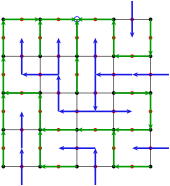
\includegraphics[]{pic-disc.pdf}
\end{center}


\subsubsection{Example}

A surface code with rough \& smooth boundary,
with parameters $n=32, m_X=15, m_Z=16, k=1.$

\begin{center}
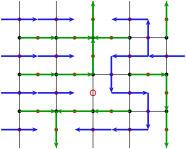
\includegraphics[]{pic-surface.pdf}
\end{center}


\subsubsection{Example}

A toric code,
with parameters $n=32, m_X=15, m_Z=15, k=2.$

\begin{center}
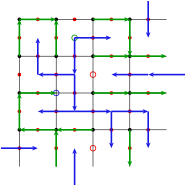
\includegraphics[]{pic-torus.pdf}
\end{center}







\bibliography{refs}{}
\bibliographystyle{abbrv}



\end{document}



